%%\documentclass[a4paper,12pt,oneside]{llncs}
\documentclass[12pt,letterpaper]{article}
\usepackage[right=2cm,left=3cm,top=2cm,bottom=2cm,headsep=0cm]{geometry}

%%%%%%%%%%%%%%%%%%%%%%%%%%%%%%%%%%%%%%%%%%%%%%%%%%%%%%%%%%%
%% Juego de caracteres usado en el archivo fuente: UTF-8
\usepackage{ucs}
\usepackage[utf8x]{inputenc}

%%%%%%%%%%%%%%%%%%%%%%%%%%%%%%%%%%%%%%%%%%%%%%%%%%%%%%%%%%%
%% Juego de caracteres usado en la salida dvi
%% Otra posibilidad: \usepackage{t1enc}
\usepackage[T1]{fontenc}

%%%%%%%%%%%%%%%%%%%%%%%%%%%%%%%%%%%%%%%%%%%%%%%%%%%%%%%%%%%
%% Ajusta maergenes para a4
%\usepackage{a4wide}

%%%%%%%%%%%%%%%%%%%%%%%%%%%%%%%%%%%%%%%%%%%%%%%%%%%%%%%%%%%
%% Uso fuente postscript times, para que los ps y pdf queden y pequeños...
\usepackage{times}

%%%%%%%%%%%%%%%%%%%%%%%%%%%%%%%%%%%%%%%%%%%%%%%%%%%%%%%%%%%
%% Posibilidad de hipertexto (especialmente en pdf)
%\usepackage{hyperref}
\usepackage[bookmarks = true, colorlinks=true, linkcolor = black, citecolor = black, menucolor = black, urlcolor = black]{hyperref}

%%%%%%%%%%%%%%%%%%%%%%%%%%%%%%%%%%%%%%%%%%%%%%%%%%%%%%%%%%%
%% Graficos 
\usepackage{graphics,graphicx}

%%%%%%%%%%%%%%%%%%%%%%%%%%%%%%%%%%%%%%%%%%%%%%%%%%%%%%%%%%%
%% Ciertos caracteres "raros"...
\usepackage{latexsym}

%%%%%%%%%%%%%%%%%%%%%%%%%%%%%%%%%%%%%%%%%%%%%%%%%%%%%%%%%%%
%% Matematicas aun más fuertes (american math dociety)
\usepackage{amsmath}

%%%%%%%%%%%%%%%%%%%%%%%%%%%%%%%%%%%%%%%%%%%%%%%%%%%%%%%%%%%
\usepackage{multirow} % para las tablas
\usepackage[spanish,es-tabla]{babel}

%%%%%%%%%%%%%%%%%%%%%%%%%%%%%%%%%%%%%%%%%%%%%%%%%%%%%%%%%%%
%% Fuentes matematicas lo mas compatibles posibles con postscript (times)
%% (Esto no funciona para todos los simbolos pero reduce mucho el tamaño del
%% pdf si hay muchas matamaticas....
\usepackage{mathptm}

%%% VARIOS:
%\usepackage{slashbox}
\usepackage{verbatim}
\usepackage{array}
\usepackage{listings}
\usepackage{multirow}

%% MARCA DE AGUA
%% Este package de "draft copy" NO funciona con pdflatex
%%\usepackage{draftcopy}
%% Este package de "draft copy" SI funciona con pdflatex
%%%\usepackage{pdfdraftcopy}
%%%%%%%%%%%%%%%%%%%%%%%%%%%%%%%%%%%%%%%%%%%%%%%%%%%%%%%%%%%
%% Indenteacion en español...
\usepackage[spanish]{babel}

\usepackage{listingsutf8}
% Para escribir código en C
% \begin{lstlisting}[language=C]
% #include <stdio.h>
% int main(int argc, char* argv[]) {
% puts("Hola mundo!");
% }
% \end{lstlisting}


\title{Examen 29/05/2019}
\author{Jesús Rodríguez Heras}

\begin{document}
	
	\maketitle
%	\begin{abstract} %Poner esto en todas las prácticas de PCTR
%%		\begin{center}
%%			\noindent
%			
%%		\end{center}
%	\end{abstract}
	\thispagestyle{empty}
	\newpage
	
%	\tableofcontents
%	\newpage
	
	%%\listoftables
	%%\newpage
	
	%%\listoffigures
	%%\newpage
	
	%%%% REAL WORK BEGINS HERE:
	
	%%Configuracion del paquete listings
	\lstset{language=bash, numbers=left, numberstyle=\tiny, numbersep=10pt, firstnumber=1, stepnumber=1, basicstyle=\small\ttfamily, tabsize=1, extendedchars=true, inputencoding=utf8/latin1, breaklines=true,literate={á}{{\'a}}1}
	
\section{Configuración inicial}
Para crear el fichero vagrant usamos el siguiente comando:
\begin{center}
	\texttt{vagrant init debian/jessie64}
\end{center}

A continuación añadimos las cuatro máquinas virtuales con sus correspondientes IPs:
\begin{itemize}
	\item VM1: 192.168.2.11
	\item VM2: 192.168.2.12
	\item VM3: 192.168.2.13
	\item VM4: 192.168.2.14
\end{itemize}

El vagrantfile quedaría de la siguiente forma:
\lstinputlisting{Vagrantfile}

\section{Cortafuegos}
Para configurar el cortafuegos para SSH (puerto 22), HTTP (puerto 80) y HTTPS (puerto 443) usaremos las siguientes reglas de IPTables en este orden:
\begin{enumerate}
	\item sudo iptables -A INPUT -p tcp --dport 22 -j ACCEPT
	\item sudo iptables -A INPUT -p tcp --dport 80 -j ACCEPT
	\item sudo iptables -A INPUT -p tcp --dport 443 -j ACCEPT
	\item sudo iptables -A INPUT -m state --state ESTABLISHED -j ACCEPT
	\item sudo iptables -A INPUT -j DROP
\end{enumerate}

Usamos dichas reglas para permitir las conexiones desde los puertos 22, 80 y 443 y denegar el resto (política por defecto).

Luego, para comprobar que los puertos están abiertos, nos dirigiremos a otra máquina virtual, por ejemplo, vm3, e instalaremos curl con:
\begin{center}
	\texttt{sudo apt-get install curl}
\end{center}

Y comprobaremos que los puertos están abiertos con:
\begin{center}
	\texttt{curl -v telnet://192.168.2.11:22/ \\
		curl -v telnet://192.168.2.11:80/ \\
		curl -v telnet://192.168.2.11:443/ \\
	curl -v telnet://192.168.2.11:79/}
\end{center}

También comprobamos el puerto 79 para ver la diferencia, ya que el 79 ha de estar cerrado. Por lo que se quedará esperando una respuesta del servidor que nunca llegará, al revés que con los otros puertos que llegamos al servidor pero no hay ningún servicio en esos puertos.

En esta imagen tenemos el resultado del curl:
\begin{figure}[h]
	\centering
	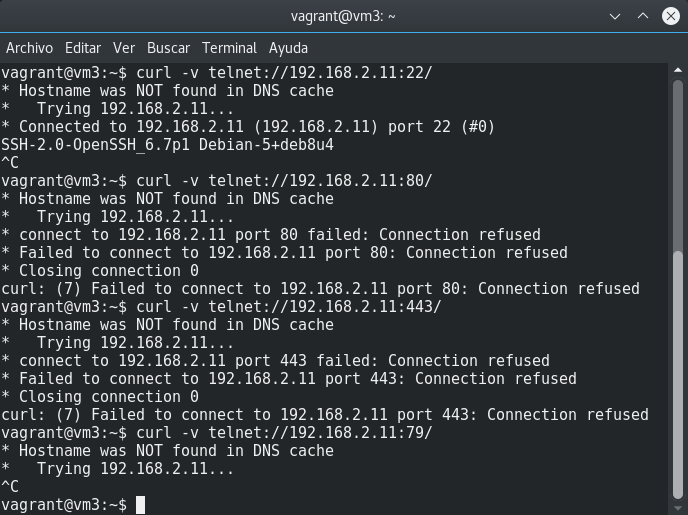
\includegraphics[scale=0.5]{Curl.png}
	\caption{Resultados del curl.}
	
\end{figure}

\section{Apache}
\subsection{Instalación de Apache}
Instalamos Apache en el servidor principal con:
\begin{center}
	\texttt{sudo apt-get update\\sudo apt-get install apache2}
\end{center}

\subsection{Instalación de PHP}
Para instalar PHP usaremos el siguiente comando:
\begin{center}
	\texttt{sudo apt-get install php5-common libapache2-mod-php5}
\end{center}

\subsection{Instalación de Webmin}
Para instalar Webmin tendremos que acceder a la página de descargas de webmin para Debian: \url{http://www.webmin.com/deb.html}.

Nos dirigimos al apartado \textit{Using the webmin APT repository}. En el archivo \texttt{/etc/apt/sources.list}
de la máquina virtual, pegamos lo siguiente:
\begin{center}
	\texttt{deb https://download.webmin.com/download/repository sarge contrib}
\end{center}

A continuación, instalamos \texttt{apt-transport-https}, actualizamos los paquetes e instalamos Webmin:
\begin{center}
	\texttt{sudo apt-get install apt-transport-https\\sudo apt-get update\\sudo apt-get install webmin}
\end{center}

\subsection{Crear los virtualhost}
Para el acceso a webmin y al servidor, previamente he configurado el fichero \texttt{/etc/hosts} de mi ordenador para que la dirección 192.168.2.11 (el servidor inicial) tenga el alias \texttt{www.jrh.ai}.
\newpage
\begin{figure}[h]
	\centering
	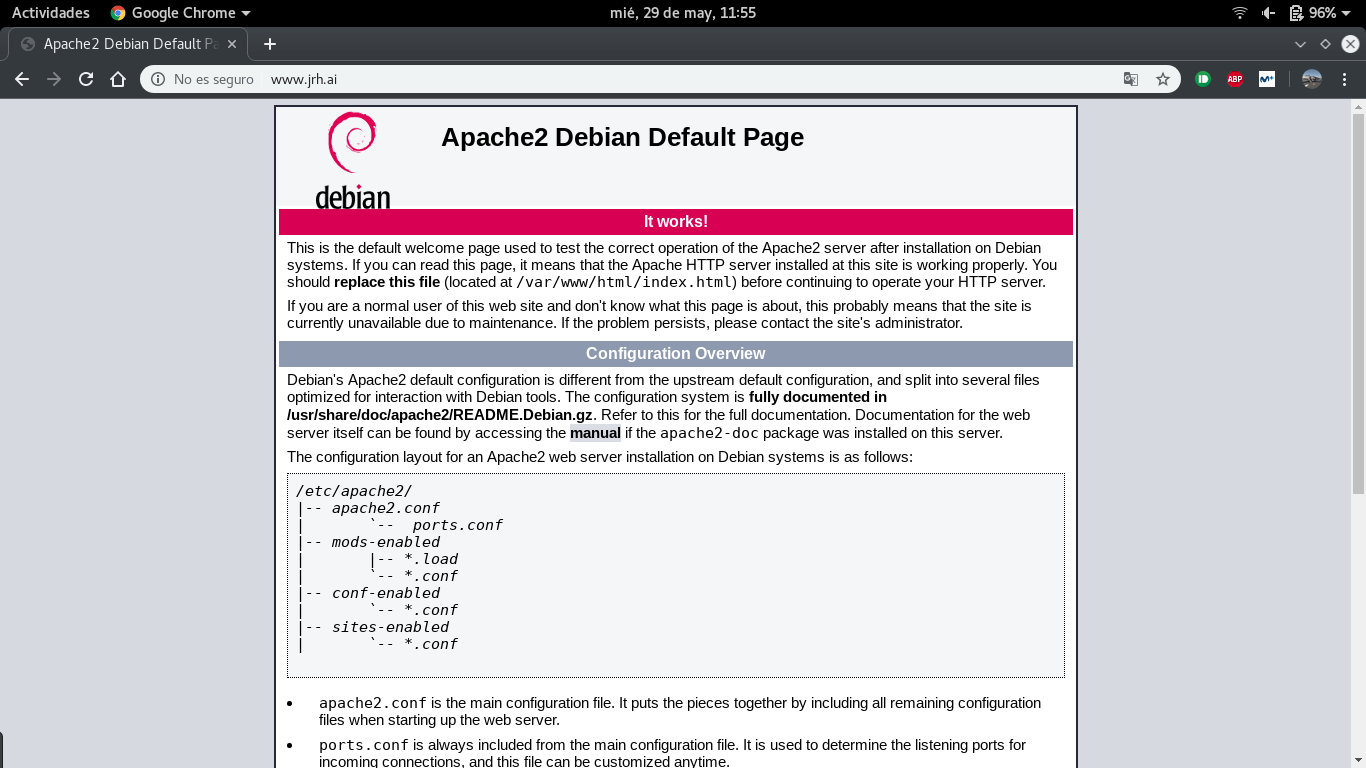
\includegraphics[scale=0.28]{Apache.png}
	\caption{Página principal de apache.}
	\label{Pagina principal de apache}
\end{figure}

Para entrar en webmin iremos a la dirección \texttt{https://jrh.ai:10000} y entraremos con usuario \texttt{vagrant} y contraseña \texttt{vagrant}.
\begin{figure}[h]
	\centering
	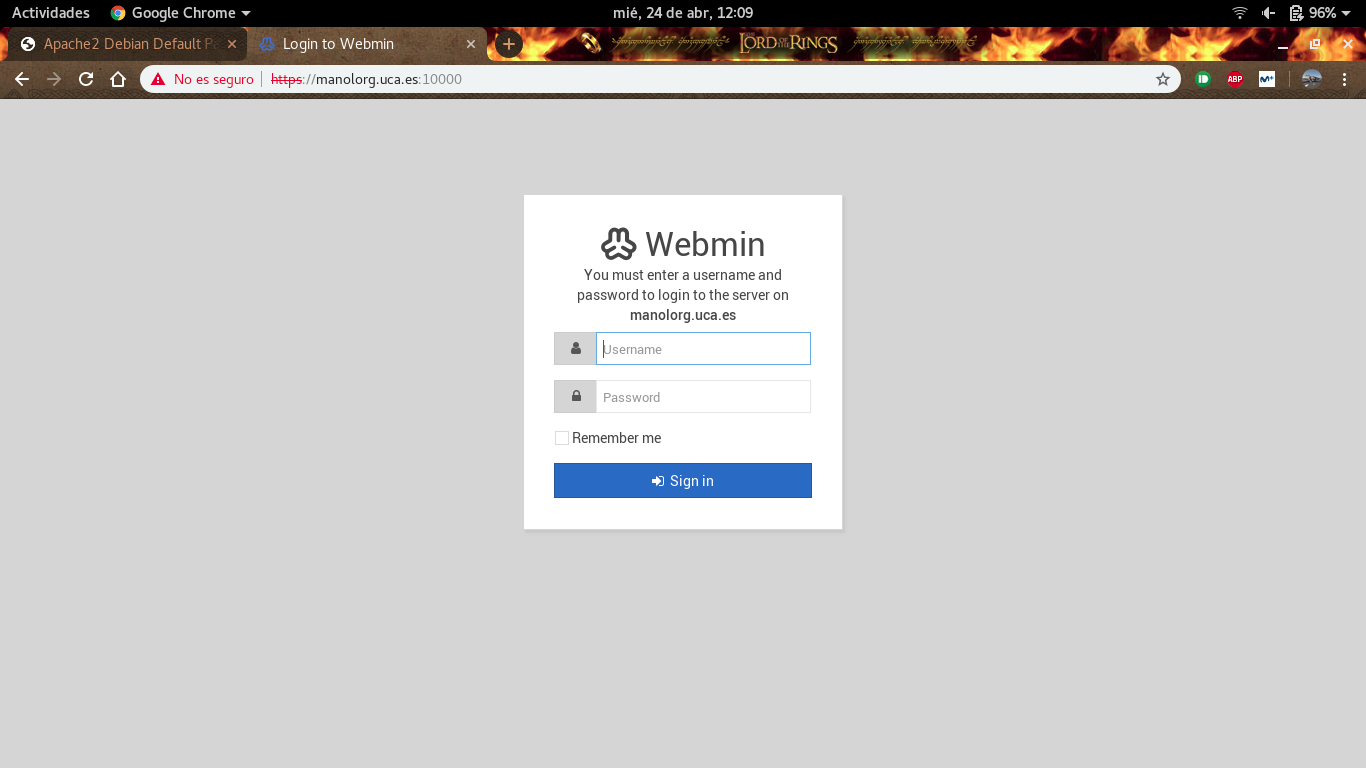
\includegraphics[scale=0.28]{Webmin.png}
	\caption{Página principal de Webmin.}
	\label{Pagina principal de Webmin}
\end{figure}

Ahora tenemos que configurar los virtualhosts. Para ello, tenemos que crear el directorio \texttt{jrh} dentro de \texttt{/var/www/} y, dentro de \texttt{/var/www/jrh/} creamos los directorios \texttt{test} y \texttt{admin}.


Luego, vamos a la pestaña ``Apache webserver'' de webmin y le damos a ``Create virtual host''. Creamos los hosts virtuales con los ``Document root'' y ``Server name'' y nos debería quedar algo tal que así:
\newpage
\begin{figure}[h]
	\centering
	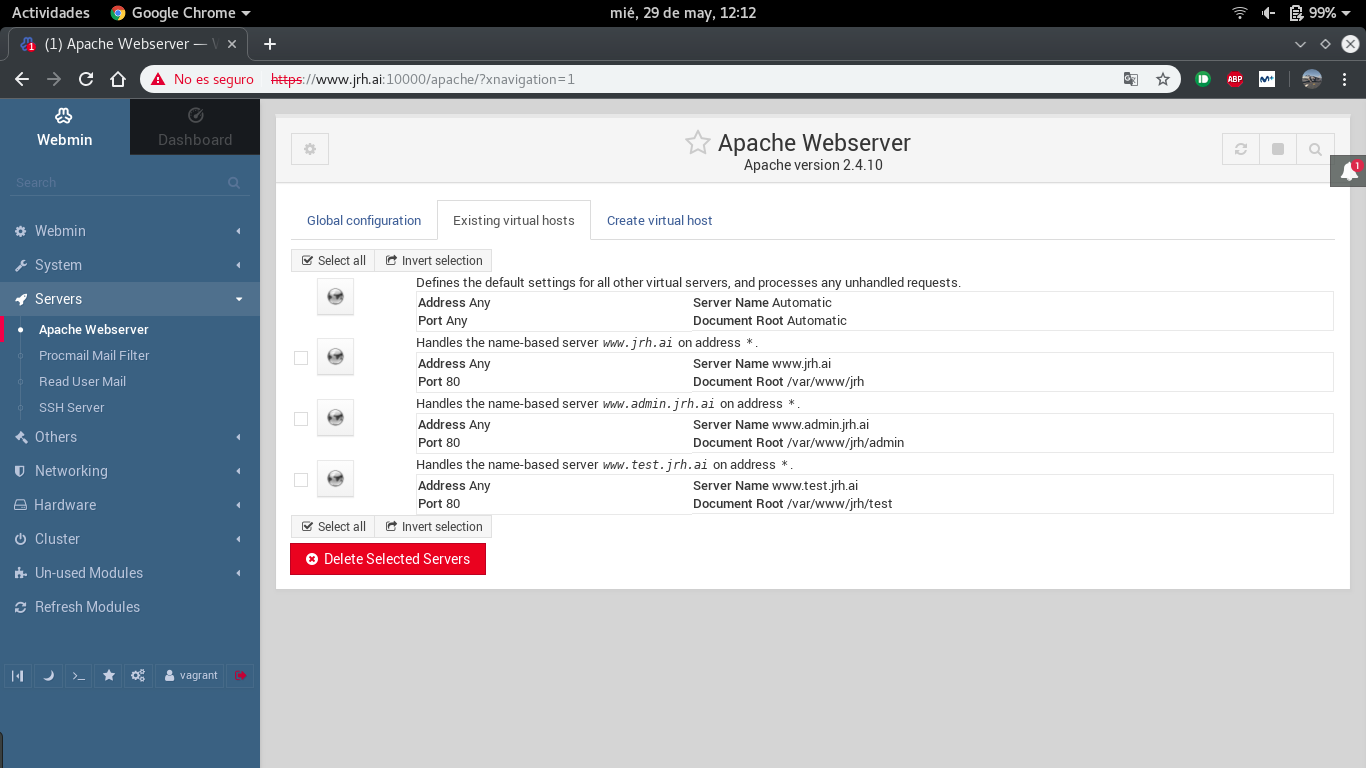
\includegraphics[scale=0.28]{ConfWebmin.png}
	\caption{Configuración de virtual hosts.}
	\label{Configuracion de virtual hosts}
\end{figure}

En el virtual host principal \texttt{www.jrh.ai} crearemos el directorio \texttt{src} que podrá ser indexado.

Para ello, creamos el directorio \texttt{/var/www/jrh/src} y, luego, entramos en el virtual host para añadir el directorio. Introducimos el path del directorio y le damos a ``Create''.

A continuación, nos dirigimos en webmin a ese directorio y en ``Document options'' marcamos la casilla de ``Selected below'' y la de ``Generate directory indexes'' y guardamos.

\begin{figure}[h]
	\centering
	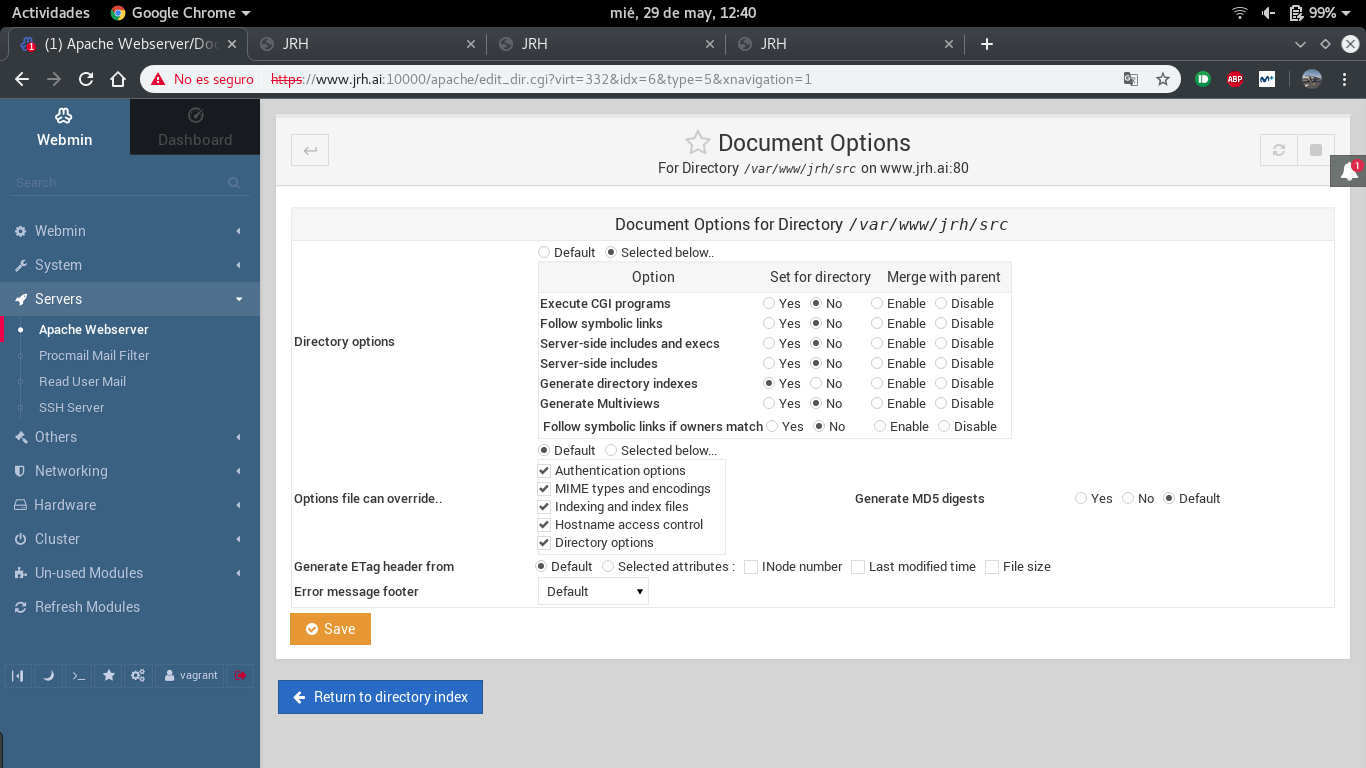
\includegraphics[scale=0.28]{Index.png}
	\caption{Directorio src indexado.}
	\label{Directorio src indexado}
\end{figure}

Para comprobar que funciona creamos algunos archivos en el directorio \texttt{/var/www/jrh/src/} y entramos mediante el navegador como en la siguiente imagen:
\newpage
\begin{figure}[h]
	\centering
	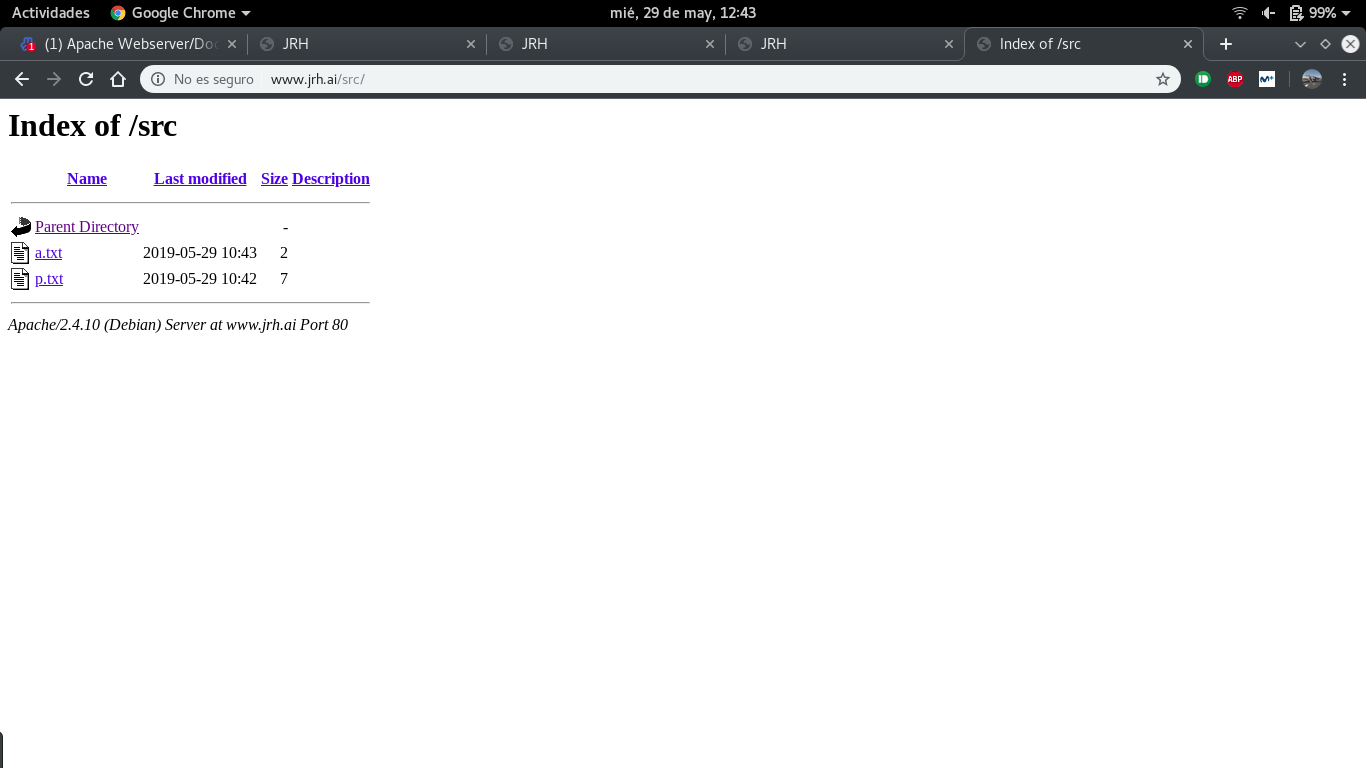
\includegraphics[scale=0.28]{src.png}
	\caption{Directorio src.}
	\label{Directorio src}
\end{figure}


\subsection{Crear una pequeña página web en cada uno de los virtualhots con tildes y demás caracteres especiales}
Para que podamos escribir tildes y caracteres especiales nos dirigimos a ``Global configuration'' y luego a ``Edit config files'' (en Webmin) y añadimos al final:
\begin{center}
	\texttt{adddefaultcharset utf-8}
\end{center}

Para ver que funcionan las tildes, crearemos el fichero \texttt{index.html} dentro del directorio \texttt{/var/www/jrh/} que contendrá el siguiente código:
\begin{lstlisting}{language=html}
	<html>
		<head>
			<title>JRH</title>
		</head>
		<body>
			<p>Página de inicio de JRH.</p>
		</body>
	</html>
\end{lstlisting}
\newpage
\begin{figure}[h]
	\centering
	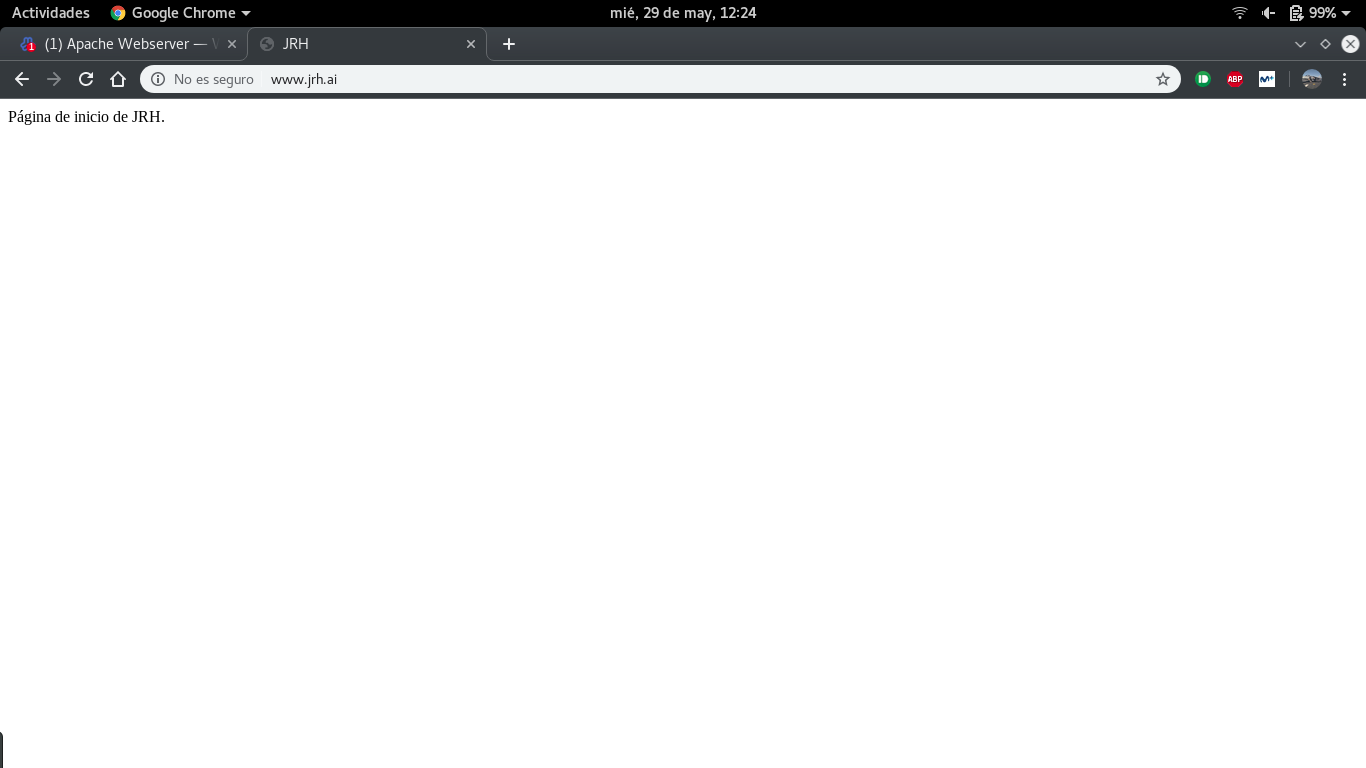
\includegraphics[scale=0.28]{IndexPHP.png}
	\caption{Página de inicio de JRH.}
	\label{Pagina de inicip de JRH}
\end{figure}

Los directorios \texttt{admin} y \texttt{test} tendrán también un código similar en su \texttt{index.html} y lo podremos ver accediendo a ellos como en la siguiente imagen:
\begin{figure}[h]
	\centering
	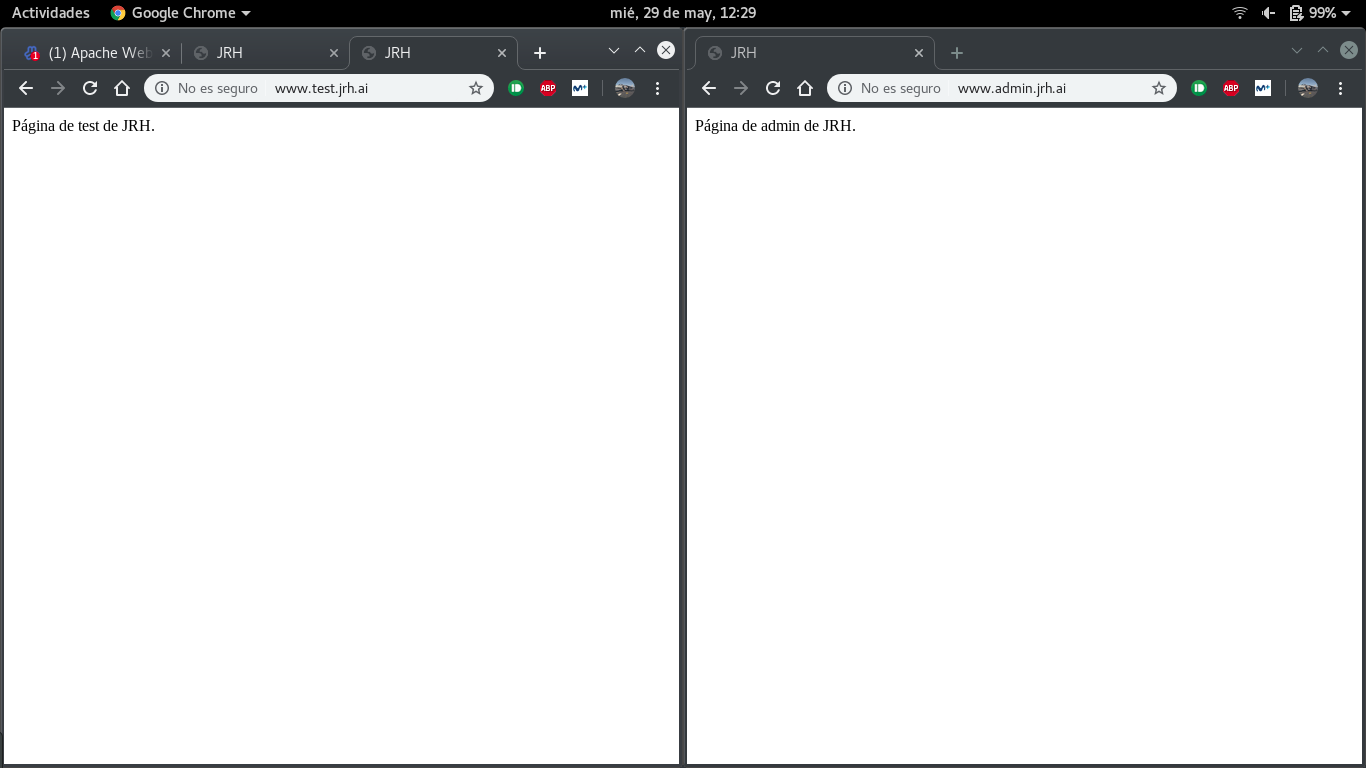
\includegraphics[scale=0.28]{DirectoriosWeb.png}
	\caption{Subdominios test y admin.}
	\label{Directorios test y admin}
\end{figure}


\subsection{Establecer la redirección}
Ahora creamos el fichero \texttt{prodList.php} en el directorio \texttt{/var/www/jrh/} que contendrá el siguiente código en PHP:
\begin{lstlisting}
	<?php
	echo 'Página del producto ' . htmlspecialchars($_GET["id"]);
	?>
\end{lstlisting}

El resultado habitual sería el siguiente (accediendo a \texttt{www.jrh.ai/prodList.php?id=002}):
\begin{figure}[h]
	\centering
	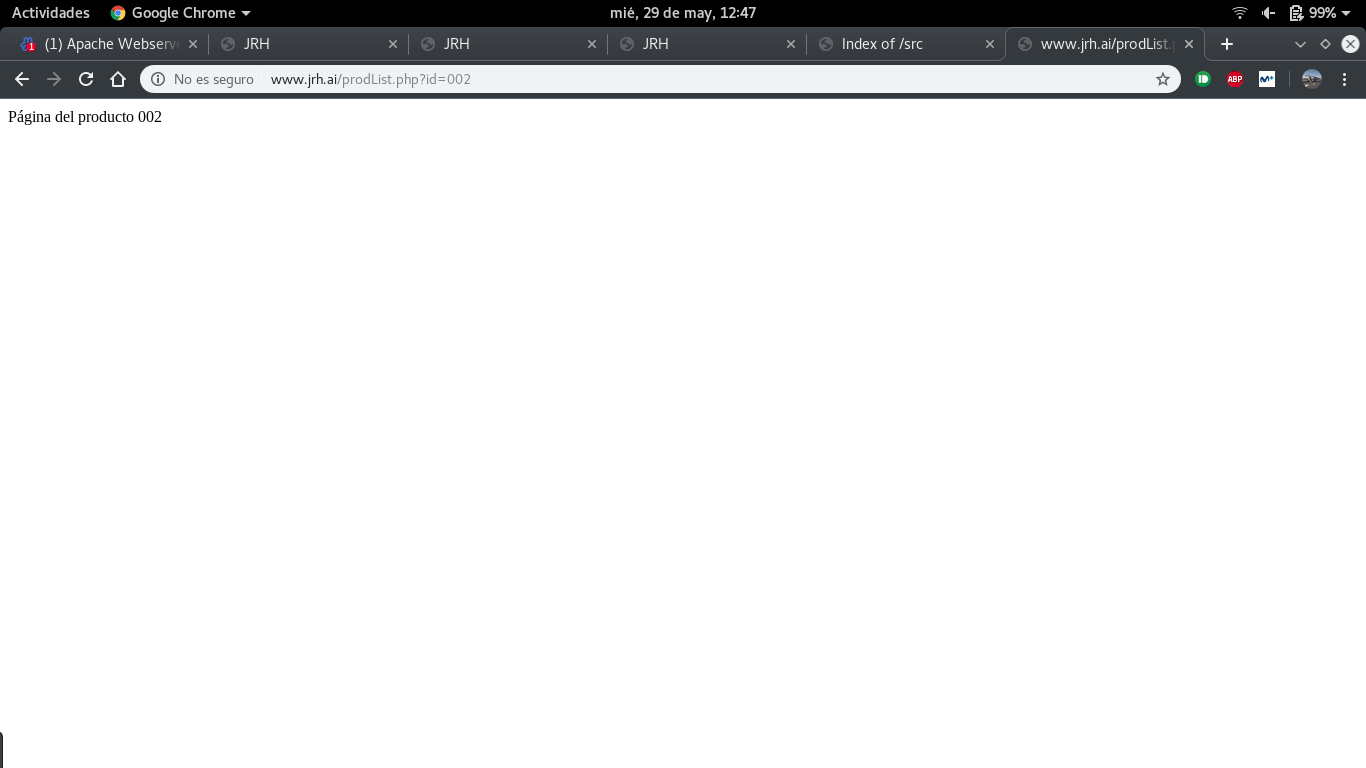
\includegraphics[scale=0.28]{prodList.png}
	\caption{prodList sin redirección.}
\end{figure}

Ahora debemos hacer la redirección para que se pueda usar un enlace más amgiable.

Para ello, habilitamos el módulo ``rewrite'' en ``Configure apache modules'' de ``Global configuration''.

Luego, añadimos la siguiente línea en el ``Edit config files'' de ``Global configuration'':
\begin{center}
	\texttt{RewriteRule ``\^/catalogo/(.*)'' ``/prodList.php?id=\$1''}
\end{center}
Tiene un acento circunflejo delante pero se me pone arriba de la barra en latex (no se por qué).\\

Para ver el resultado con la redirección entramos en \texttt{www.jrh.ai/catalogo/002}:
\newpage
\begin{figure}[h]
	\centering
	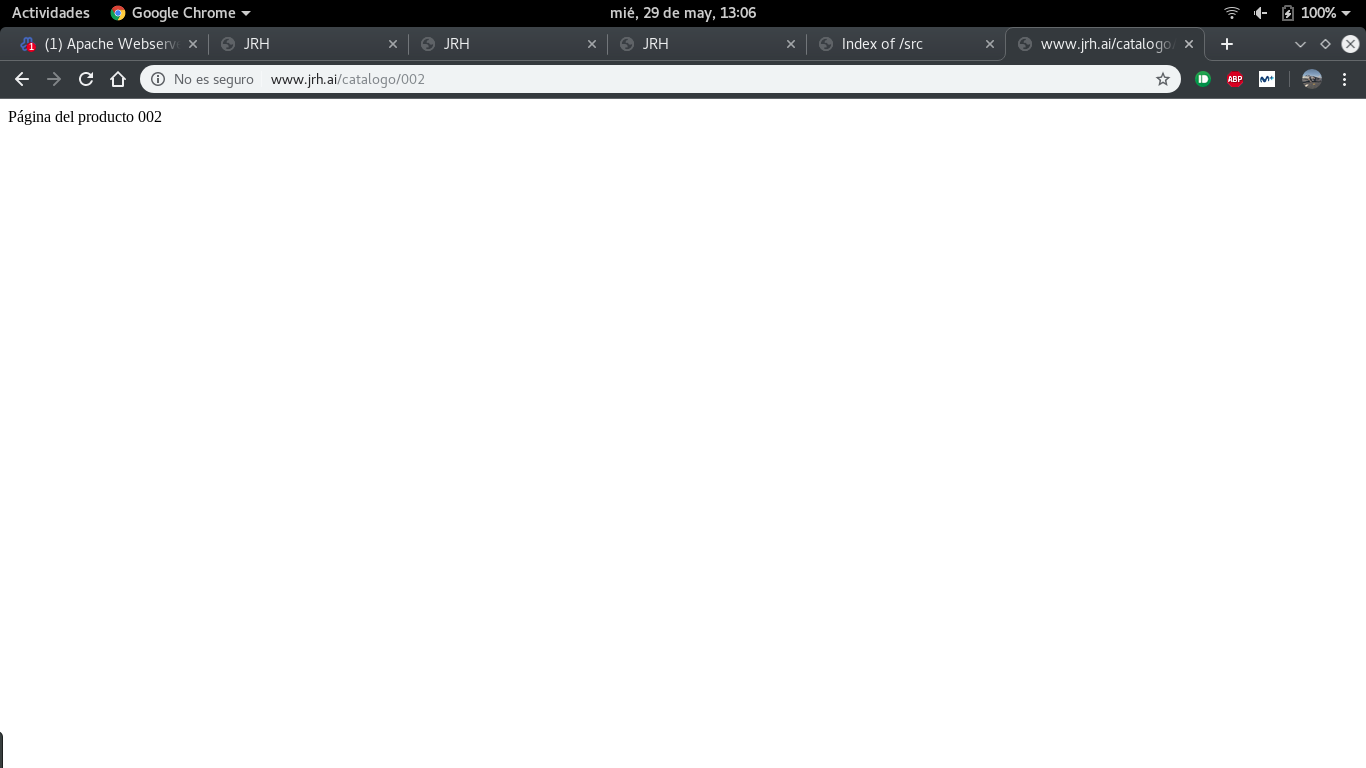
\includegraphics[scale=0.28]{Catalogo.png}
	\caption{Catalogo con redirección.}
	\label{Catalogo con redireccion}
\end{figure}

Ahora expondré los ficheros de directivas:
\begin{figure}[h]
	\centering
	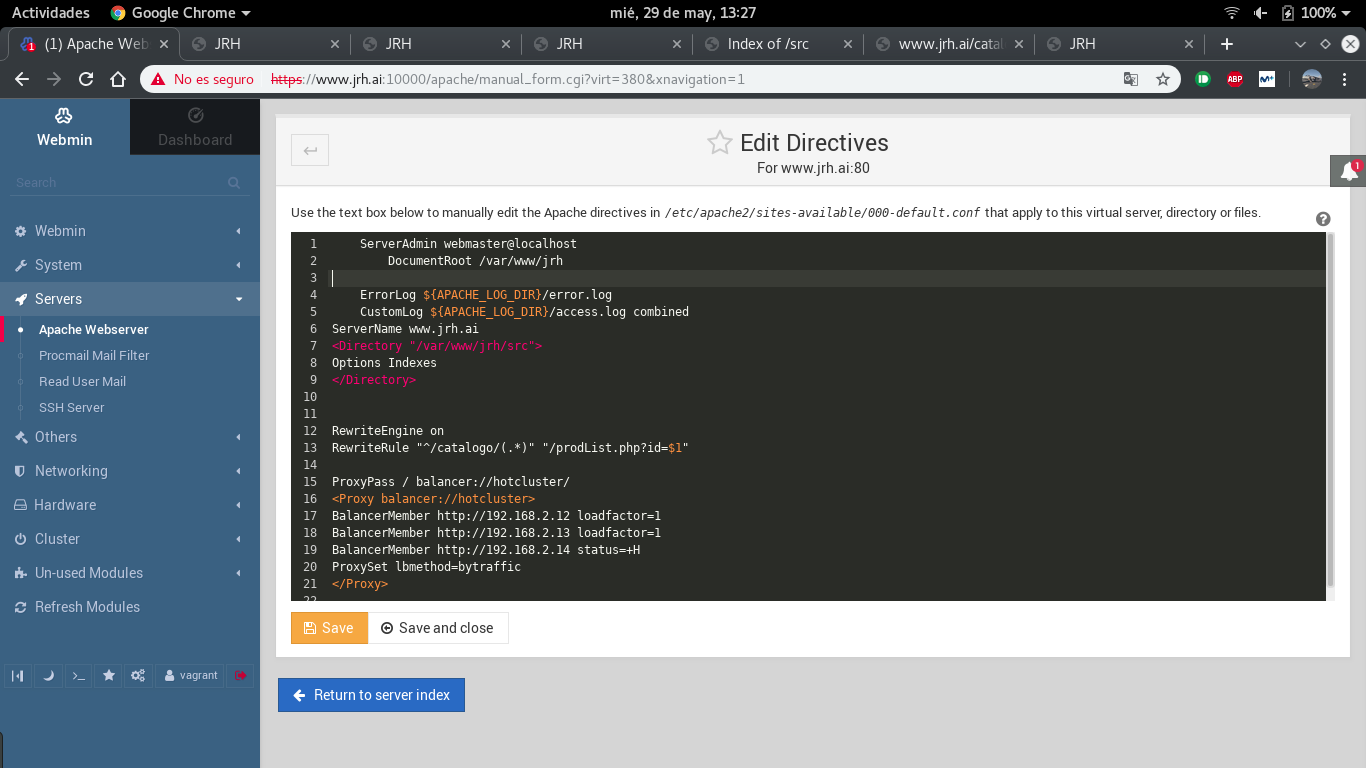
\includegraphics[scale=0.28]{DirectivasPPAL.png}
	\caption{Directivas jrh.}
	\label{Directivas jrh}
\end{figure}

\newpage
\begin{figure}[h]
	\centering
	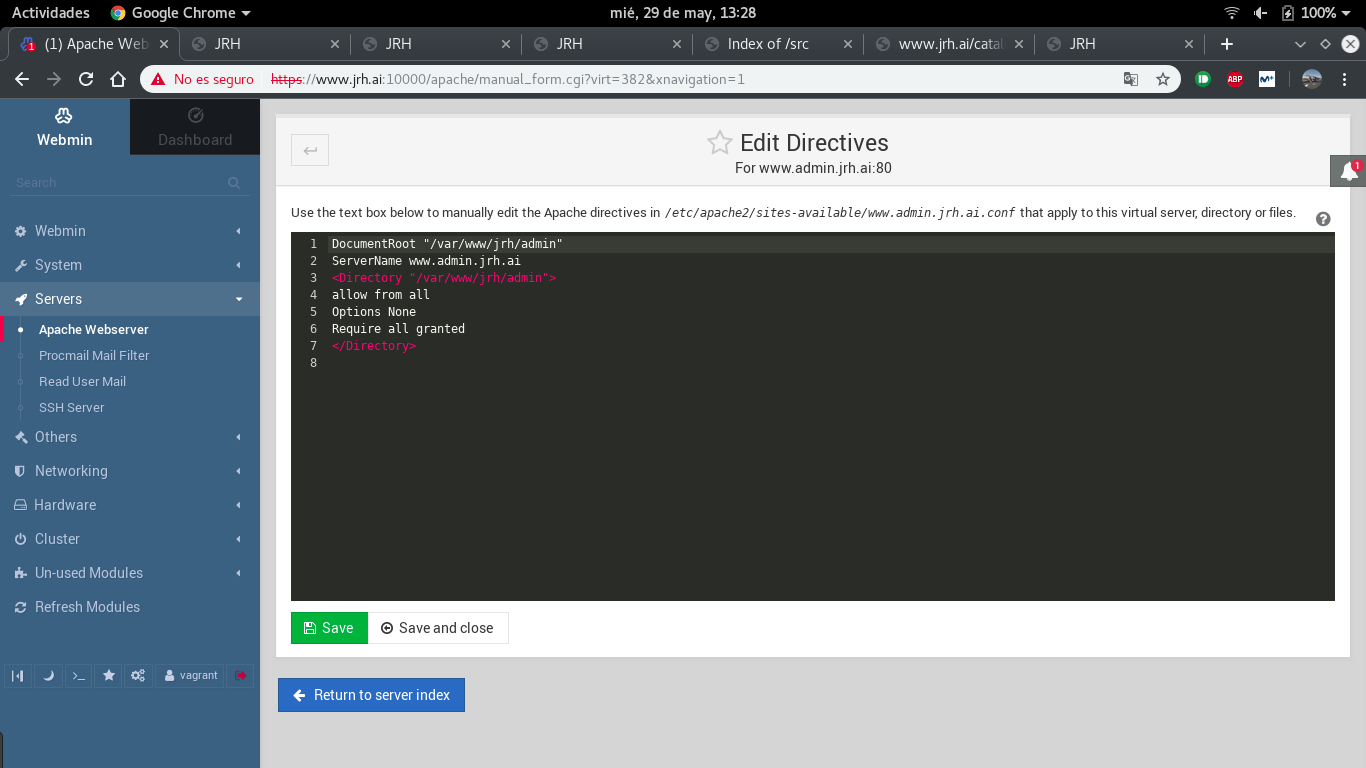
\includegraphics[scale=0.28]{DirectivasAdmin.png}
	\caption{Directivas admin.}
	\label{Directivas admin}
\end{figure}

\begin{figure}[h]
	\centering
	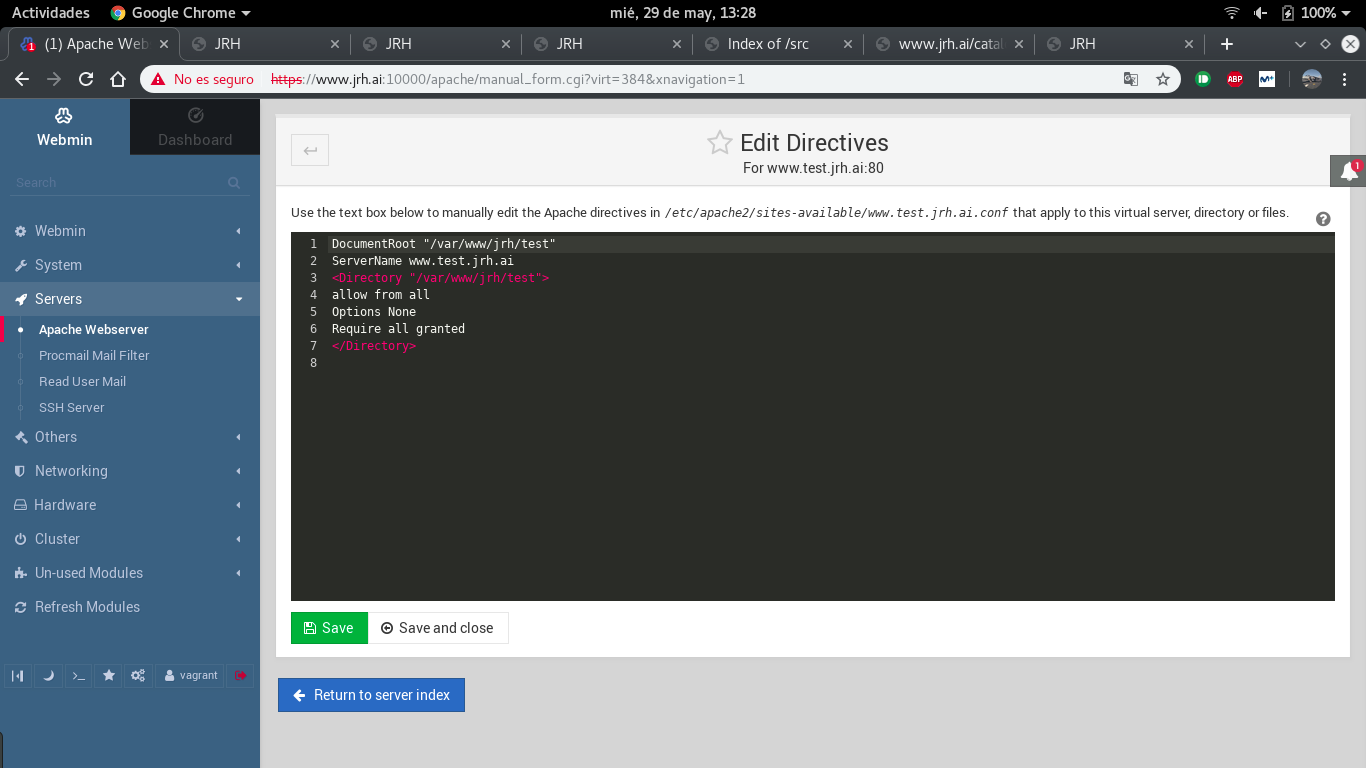
\includegraphics[scale=0.28]{DirectivasTest.png}
	\caption{Directivas test.}
	\label{Directivas test}
\end{figure}

\section{Configuración avanzada de Apache}
Como en este examen no se ha configurado el servidor DNS, le pondremos directamente la dirección IP de los otros nodos.

Para hacer el balanceo de carga, debemos tener instalado Apache en todos los nodos con:
\begin{center}
	\texttt{sudo apt-get install apache2}
\end{center}

Para comprobarlo modificaremos el fichero \texttt{index.html} de la siguiente forma:
\begin{lstlisting}
	<html>
	<head>
	<title>JRH</title>
	</head>
	<body>
	<p>Página de inicio de JRH en nodo 1.</p>
	</body>
	</html>
\end{lstlisting}

Para los nodos 2 y 3 estará modificado también.

Ahora, nos dirigimos a webmin y habilitamos los siguientes modulos de Apache:
\begin{itemize}
	\item lbmethod\_bybusyness
	\item lbmethod\_byrequests
	\item lbmethod\_bytrafic
	\item lbmethod\_heartbeat
	\item proxy\_balancer
	\item proxy\_html
	\item proxy\_http
\end{itemize}

Luego, nos dirigimos al host virtual por defecto de la máquina que actúa como balanceador y, en “Edit directives” ponemos lo siguiente:\\

\noindent
\texttt{ProxyPass / balancer://hotcluster/
	<Proxy balancer://hotcluster>
	BalancerMember http://192.168.2.12 loadfactor=1
	BalancerMember http://192.168.2.13 loadfactor=1
	BalancerMember http://192.168.2.14 status=+H
	ProxySet lbmethod=bytraffic
	</Proxy>}

\newpage
Para comprobar que funciona, solo debemos entrar dos veces en la página para que podamos ver lo siguiente:
\begin{figure}[h]
	\centering
	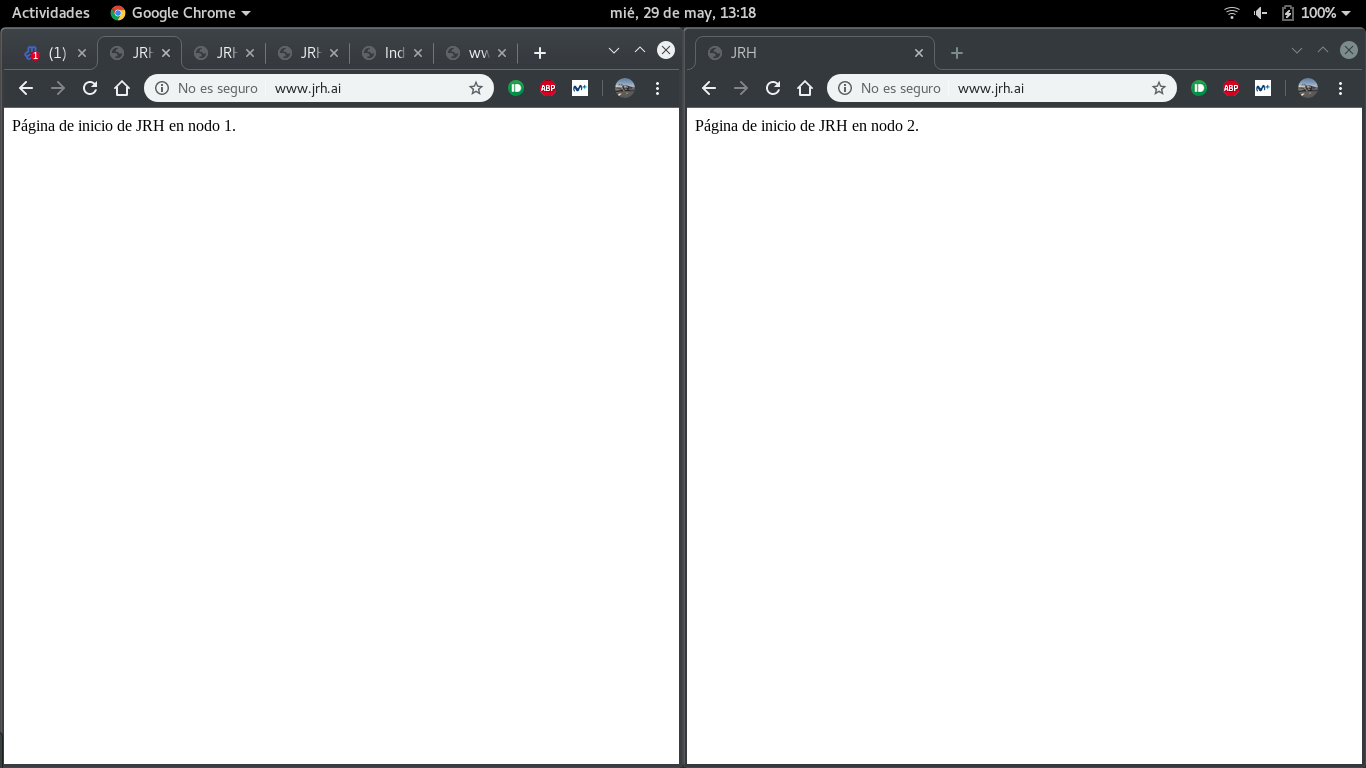
\includegraphics[scale=0.28]{Balanceo.png}
	\caption{Balanceo de carga.}
	\label{Balanceo de carga}
\end{figure}
\end{document}